\section{Discussion and Conclusion}\label{sec:dis}


% From \autoref{tab:afrho} we can conclude that the comet C/2019 L3 is very active due to its high $A(0)f\rho$ values during the observational run, while C/2020 P3 is less active since its $A(0)f\rho$ values are only about {\SI{10}{\percent}} of that of C/2019 L3. 
Comparing $A(0)f\rho$ values with that of other LPCs, just as Fig.~\ref{fig:afrho-ref} shown, C/2019 L3 is very active at heliocentric distance of $\thicksim${\qty{4}{\astronomicalunit}}, and C/2020 P3 is moderately active at heliocentric distance of $\thicksim${\qty{7}{\astronomicalunit}}. 
Moreover, % 在此只写活动性显现出异常, 不作过度猜测
it can be seen from Fig.~\ref{fig:a0frho-c2019} that during the observation period, the R-band $A(0)f\rho$ values of comet C/2019 L3, measured at an aperture of {\SI{e4}{\km}}, showed a trend of initially decreasing followed by an increase. This could be attributed to a previous outburst, followed by a gradual increase in activity as it approaches perihelion. 
On the other hand, 
the BC-band $A(0)f\rho$ value of C/2019 L3 up to \SI{24710 +- 125}{\cm} on \DTMdate{2022-1-19} posted on The Astronomer's Telegram\footnote{\href{https://www.astronomerstelegram.org/?read=15186}{https://www.astronomerstelegram.org/?read=15186}}, with heliocentric distance $r = \SI{3.56}{\astronomicalunit}$ and geocentric distance $\Delta = \SI{2.61}{\astronomicalunit}$, indicates that C/2019 L3 appears very active near the perihelion. 


% 与其他LPC比较,相位角均校正至0
\begin{figure}
    \centering
    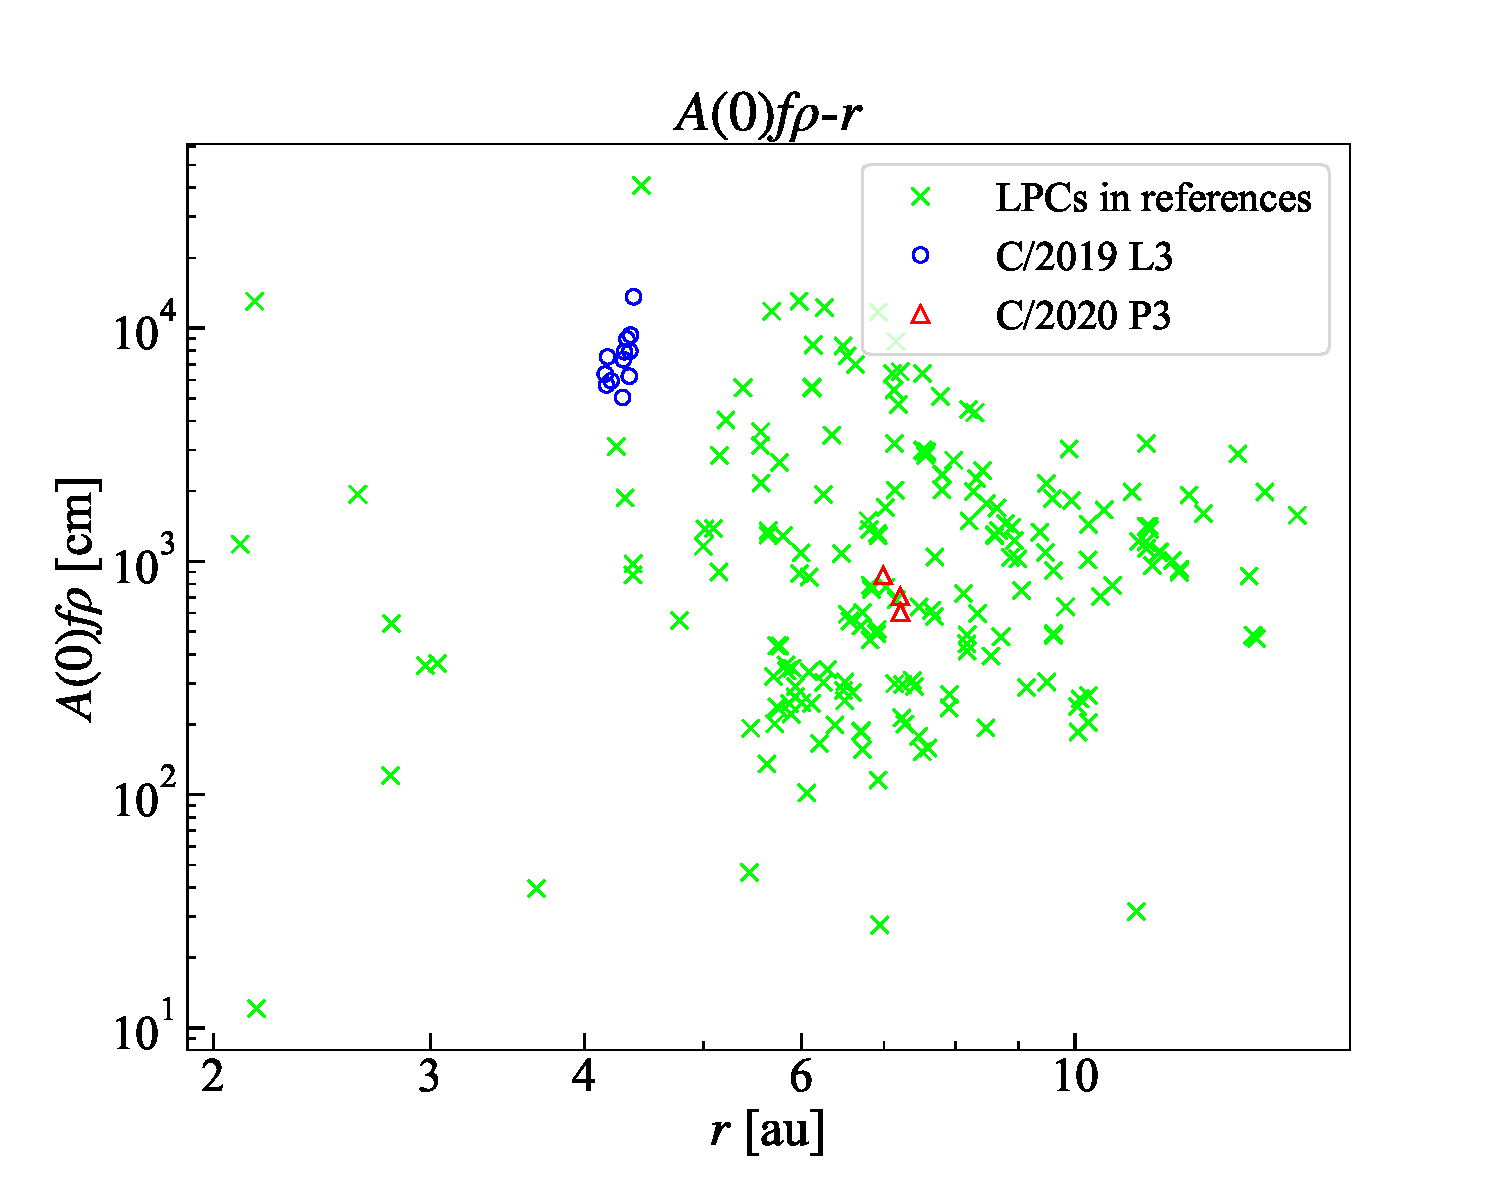
\includegraphics[width=\columnwidth]{a0frho-r.pdf}
    \caption{$A(0)f\rho$ values measured in this work compared with that of other LPCs in  literature by \citet{mazzotta_epifani_observational_2014}, \citet{garcia_photometry_2021}, \citet{garcia_observational_2020}, \citet{rousselot_monitoring_2014}, \citet{meech_activity_2009}, \citet{sarneczky_activity_2016}, \citet{solontoi_ensemble_2012}, and \citet{szabo_spectrophotometry_2002}. All data have been adjusted to phase angle \ang{0}. }\label{fig:afrho-ref}
\end{figure}% data amount error

\begin{figure}
    \centering
    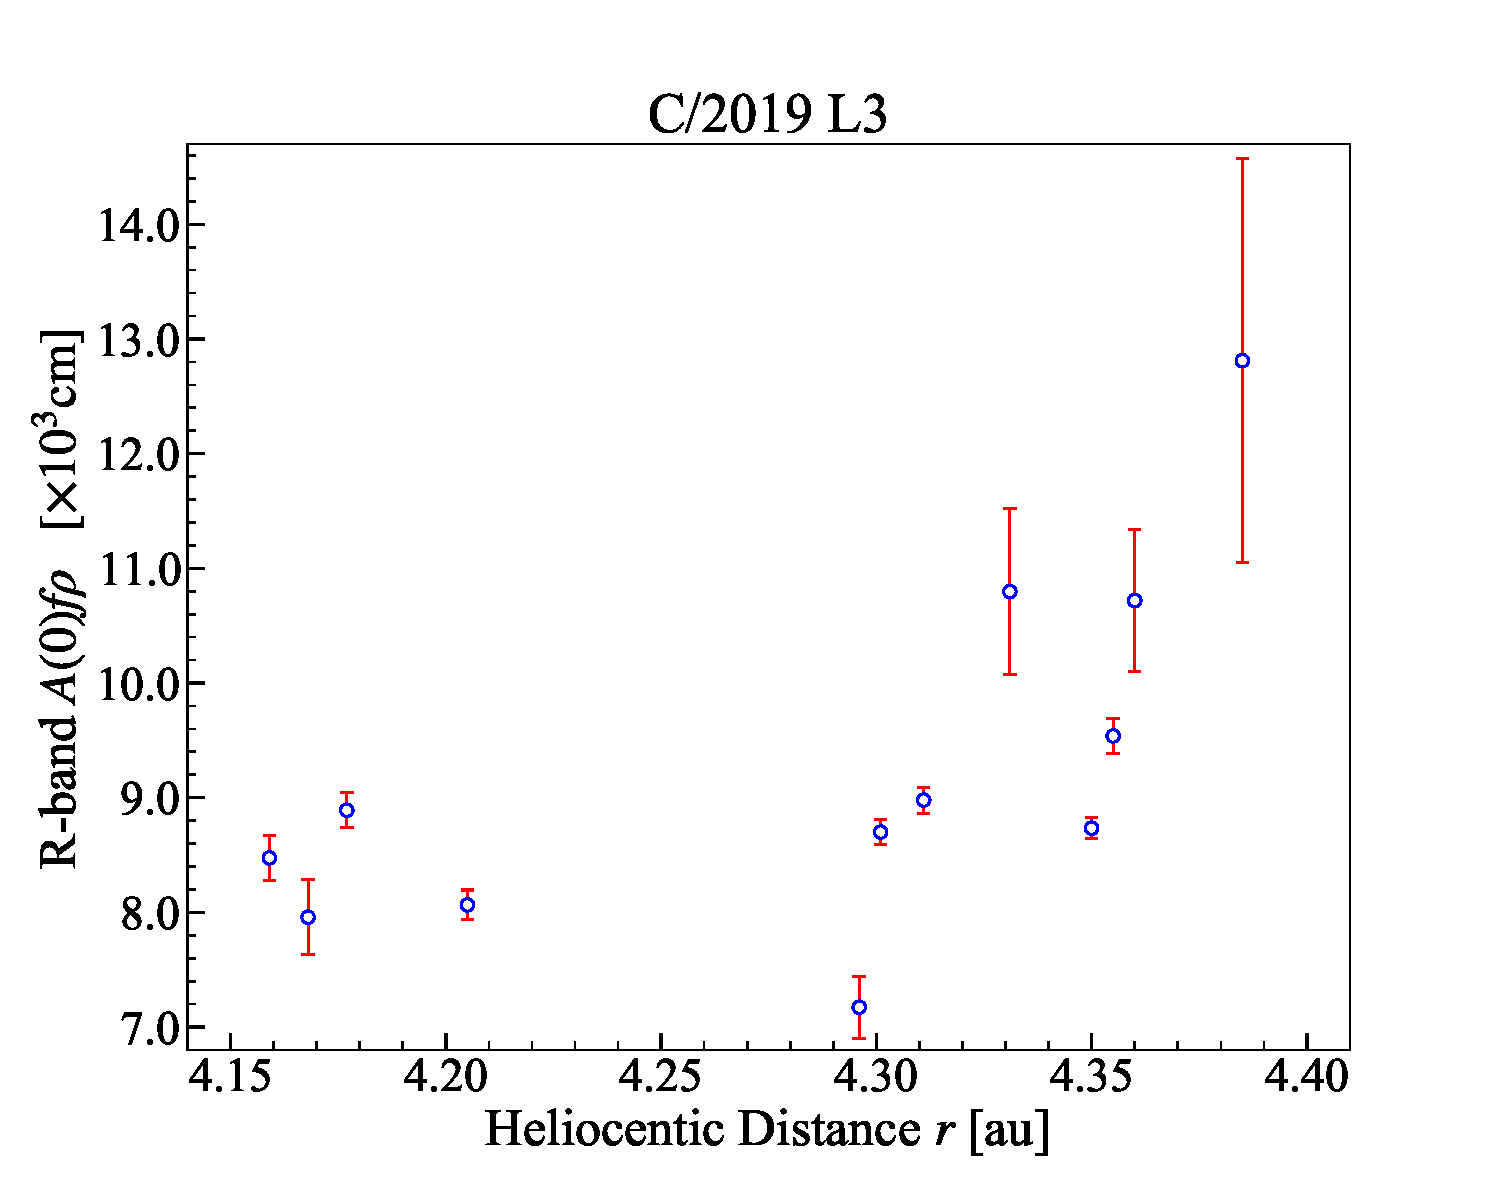
\includegraphics[width=\columnwidth]{a0frho-r-C2019L3-new.pdf}
    \caption{R-band $A(0)f\rho$ values of C/2019 L3 as a function of heliocentric distance. }\label{fig:a0frho-c2019}
\end{figure}

According to the study by \cite{ramirez_ubvric_2012}, the solar colors are as follows: 
${(\mathrm{B} - \mathrm{V})}_{\odot} = \num{0.653 +- 0.005}$, 
${(\mathrm{V} - \mathrm{R})}_{\odot} = \num{0.352 +- 0.007}$, and 
${(\mathrm{R} - \mathrm{I})}_{\odot} = \num{0.350 +- 0.009}$. 
The average color indices of two Long-period comets and three dynamically new comets were calculated by \cite{meech_activity_2009} to be 
$\langle \mathrm{B} - \mathrm{V} \rangle = \num{0.76 +- 0.01}$ and 
$\langle \mathrm{V} - \mathrm{R} \rangle = \num{0.43 +- 0.01}$, 
with their heliocentric distances ranging from \SIrange{5.8}{14.0}{\astronomicalunit}. 
\cite{solontoi_ensemble_2012} studied six Long-period comets within \SI{5}{\astronomicalunit} of the Sun and obtained the average color indices of 
$\langle \mathrm{B} - \mathrm{V} \rangle = \num{0.687 +- 0.005}$ and 
$\langle \mathrm{V} - \mathrm{R} \rangle = \num{0.443 +- 0.003}$. 
\cite{jewittCOLORSYSTEMATICSCOMETS2015} investigated Long-period comets with large range of heliocentric distances (\SIrange{1.875}{17.982}{\astronomicalunit}), and the average color indices were found to be 
$\langle \mathrm{B} - \mathrm{V} \rangle = \num{0.78 +- 0.02}$, 
$\langle \mathrm{V} - \mathrm{R} \rangle = \num{0.47 +- 0.02}$, and 
$\langle \mathrm{R} - \mathrm{I} \rangle = \num{0.42 +- 0.03}$. 


Fig.~\ref{fig:color-color} is the $\langle \mathrm{B}-\mathrm{V} \rangle$ versus $\langle \mathrm{V}-\mathrm{R} \rangle$ plot of C/2019 L3, C/2020 P3 and other LPCs. 
The color index of the Sun \citep{ramirez_ubvric_2012} is marked as a red circle with dot. 
As we can see, the $\langle \mathrm{B} - \mathrm{V} \rangle$ colors of two comets are redder than the Sun, while the $\langle \mathrm{V} - \mathrm{R} \rangle$ colors of them are bluer than the Sun. 
Compared with LPCs in other works, the $\langle \mathrm{B} - \mathrm{V} \rangle$ color of C/2019 L3 is consistent with them, while the $\langle \mathrm{V} - \mathrm{R} \rangle$ color of C/2019 L3 is significantly bluer than them. For C/2020 P3, the $\langle \mathrm{B} - \mathrm{V} \rangle$ color is redder while the $\langle \mathrm{V} - \mathrm{R} \rangle$ color is bluer. 
In general, the color indices of the two LPCs studied in this work differ from those of other LPCs. 


% V-R随日心距呈现变蓝的趋势, 在4au左右CO2的升华作用较明显, 因此, C/2019 L3的活动性可能是由于CO2的升华导致

\begin{figure}
    \centering
    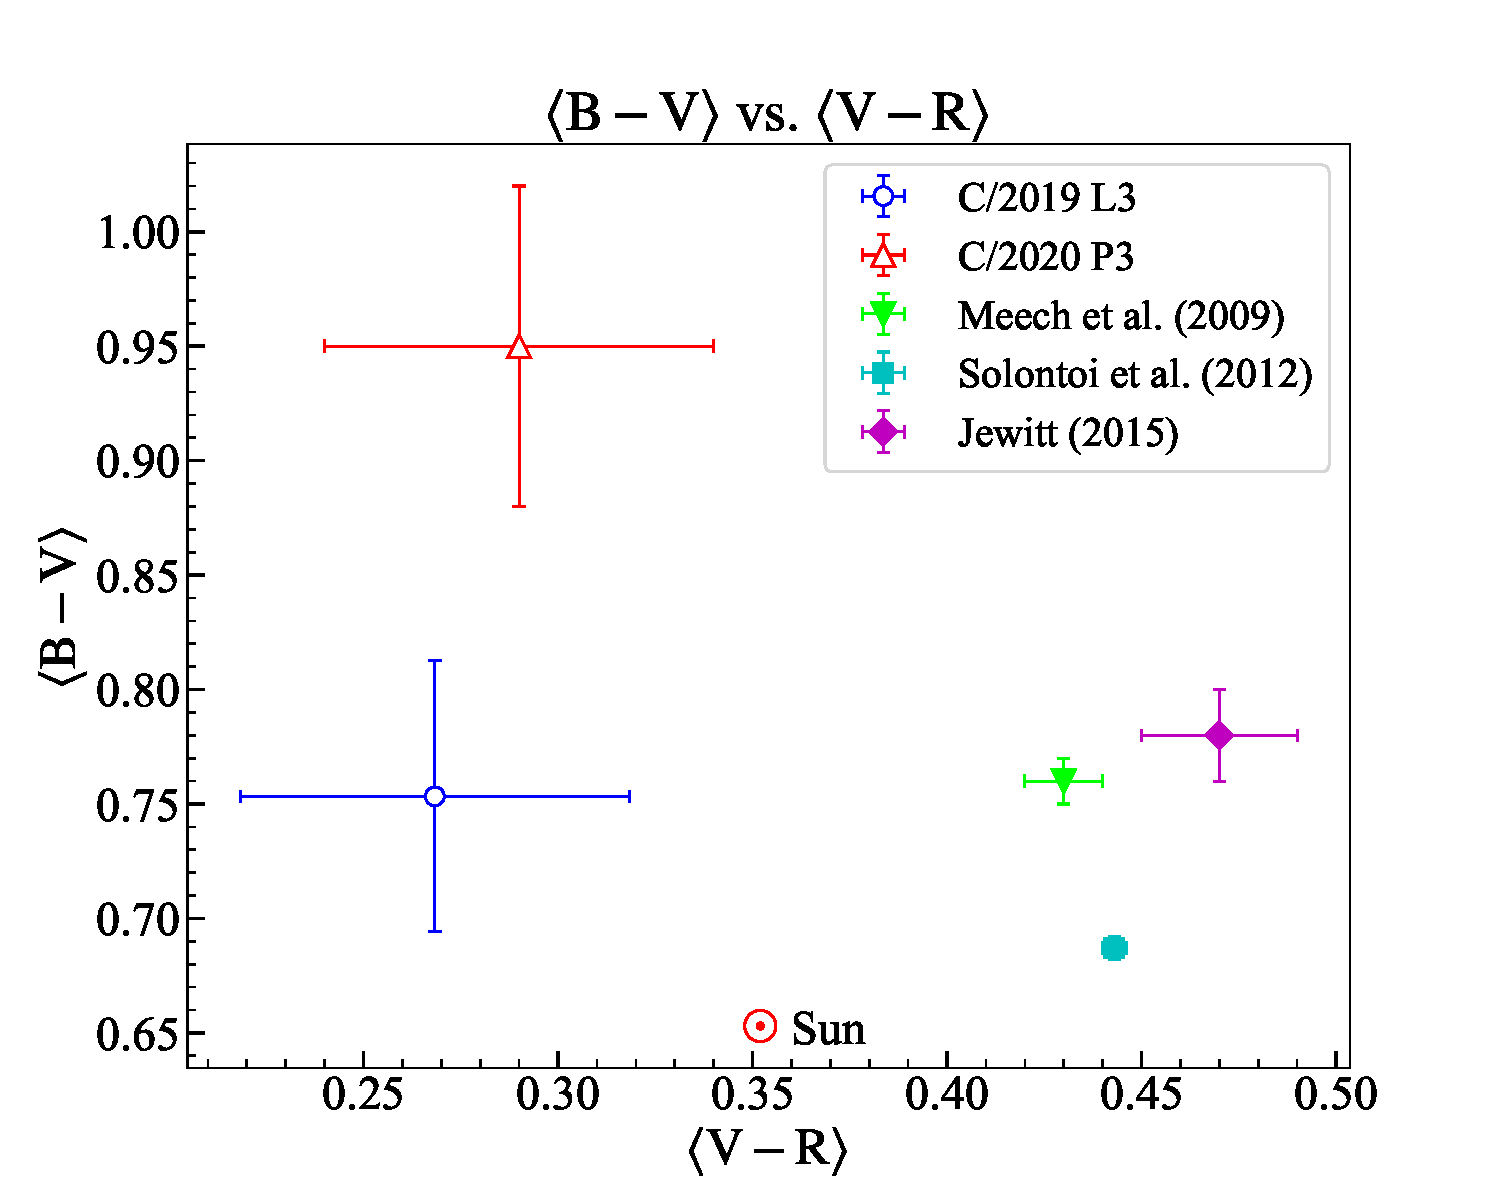
\includegraphics[width=\linewidth]{color-color.pdf}
    \caption{Color indices $\langle \mathrm{B-V} \rangle$ versus $\langle \mathrm{V-R} \rangle$ plot of Long-period comets}\label{fig:color-color}
\end{figure}

In summary, we present the observational results of comets C/2019 L3 and C/2020 P3. The conclusions are as follows: 
\begin{enumerate}
    \item For comet C/2019 L3, A fan-shape structure can be observed in the northeast direction. This feature is visible in both V and R filters. 
    \item The average gradient value  of the surface brightness profile of comet C/2019 L3 is \num{-1.66}, suggesting a nonsteady coma. 
    \item The R-band $A(0)f\rho$ values of C/2019 L3 range from {\qty{5043 +- 244}{\cm}} to {\qty{13611 +- 1874}{\cm}}, and those of C/2020 P3 range from {\qty{606 +- 31}{\cm}} to {\qty{869 +- 20}{\cm}}. Compared to other works, the $A(0)f\rho$ of C/2019 L3 is relatively high at $\thicksim${\qty{4}{\astronomicalunit}}, while that of C/2020 P3 is moderate at $\thicksim${\SI{7}{\astronomicalunit}}. The R-band $A(0)f\rho$ values of C/2019 L3 tend to decrease first and then increase, so it is possible that comet C/2019 L3 experienced an outburst event in the past, and it was still active after this stage. 
    \item The average colors for C/2019 L3 are  
        $\langle \mathrm{B-V} \rangle = \num{0.75 +- 0.06}$, 
        $\langle \mathrm{V-R} \rangle = \num{0.27 +- 0.05}$, and 
        $\langle \mathrm{R-I} \rangle = \num{0.22 +- 0.05}$,  
        while the colors for C/2020 P3 are 
        $\mathrm{B-V} = \num{0.95 +- 0.07}$, 
        $\langle \mathrm{V-R} \rangle = \num{0.29 +- 0.05}$, and 
        $\mathrm{R-I} = \num{0.21 +- 0.05}$. 
        The $\mathrm{B-V}$ colors of C/2019 L3 and C/2020 P3 are redder than the Sun, while the $\mathrm{V-R}$ and $\mathrm{R-I}$ colors of them are bluer than the Sun. Compared to other Long-period comets, both C/2019 L3 and C/2020 P3 exhibit distinct differences in their color indices. The reddening of C/2019 L3 calculated from B-band $Af\rho$ and R-band $Af\rho$ exhibits variations during the observational runs, from {\qty{13.75 +- 1.07}{\percent/\kilo\angstrom}} to {\qty{-15.69 +- 0.37}{\percent/\kilo\angstrom}} with an average value of {\qty{0.94 +- 0.23}{\percent/\kilo\angstrom}}. This could be attributed to  variations in the composition of the coma. As for C/2020 P3, the reddening could only be calculated for the date of \DTMdate{2021-5-12}, yielding a value of {\qty{-6.65 +- 0.01}{\percent/\kilo\angstrom}}. 
\end{enumerate}
